\documentclass[letterpaper,10pt]{article}

\usepackage[utf8]{inputenc}
\usepackage[spanish]{babel}
\usepackage{fontenc}
\usepackage[dvipdfmx]{graphicx}
\usepackage{bmpsize,wrapfig,xcolor}
\usepackage{fullpage}
\usepackage{amssymb}
\usepackage[hidelinks]{hyperref}

% Para evitar que se indente solo a cada rato
\setlength\parindent{0pt}

\begin{document}
	\begin{titlepage}

		\begin{wrapfigure}{R}{0.3\textwidth}
			
\includegraphics[width=0.3\textwidth]{logoFCFM.png}
		\end{wrapfigure}

		\noindent \phantom - % "Hax" para que quede alineada la imagen con el texto

		Universidad de Chile

		Facultad de Ciencias Físicas y Matemáticas

		Depto. de Ciencias de la Computación

		CC4102 - Diseño y Análisis de Algoritmos

		\vfill

		\begin{center}
			\begin{Huge}
				{\textbf{Tarea 1}}
			\end{Huge}
		\end{center}

		\vfill

		\begin{flushright}
			\begin{tabular}{lll}
				Integrantes	&:	& Rodrigo Delgado\\
						&	& Belisario Panay\\
						&	& Gabriel Sanhueza\\
				Profesor	&:	& Gonzalo Navarro\\
				Ayudante	&:	& Sebastián Ferrada\\
				Auxiliar	&:	& Jorge Bahamondes\\
			\end{tabular}
		\end{flushright}

	\end{titlepage}

	% % % % % % % % % % % % % % % % % % % % % % % % % % % % % % % % % % % % % % % % % % % % % % % % % % % % % % % % % % % % % % % % % % % % % % % % % % % % % % % % % % % % % % % % % %
	\newpage
	% % % % % % % % % % % % % % % % % % % % % % % % % % % % % % % % % % % % % % % % % % % % % % % % % % % % % % % % % % % % % % % % % % % % % % % % % % % % % % % % % % % % % % % % % %

	\tableofcontents

	% % % % % % % % % % % % % % % % % % % % % % % % % % % % % % % % % % % % % % % % % % % % % % % % % % % % % % % % % % % % % % % % % % % % % % % % % % % % % % % % % % % % % % % % % %
	\newpage
	% % % % % % % % % % % % % % % % % % % % % % % % % % % % % % % % % % % % % % % % % % % % % % % % % % % % % % % % % % % % % % % % % % % % % % % % % % % % % % % % % % % % % % % % % %

	\section{Introducción}

	\subsection{Problema a resolver}

	Los R-trees son un tipo de árbol que se maneja en memoria secundaria, el cual contiene rectángulos como información. El problema a resolver consiste en implementar un R-Tree,
	una herramienta de búsquedas de rectángulos y 2 heurísticas de inserción de rectángulos en el R-Tree.

	En particular, se busca evaluar el impacto entre distintas versiones de \textit{inserción} que manejan una versión específica de manejo de \textit{overflow} (para este caso,
	\textit{Linear Split} y \textit{Greene Split}.

	\subsection{Hipótesis}

	\subsubsection*{Especificaciones de la máquina utilizada}

	\begin{itemize}
		\item Procesador: Intel \textregistered Core \textregistered i5-4570 @ 3.20GHz
		\item Arquitectura: x86\_64
		\item Número de CPUs: 4
		\item Número de Threads: 4
		\item Memoria RAM: 8192 KB
		\item Tamaño de página de disco: M = 2048 bytes ($\ulcorner40\% M\urcorner = 820$)
		\item Sistema Operativo: Elementary O.S. 0.4 Loki
		\item Lenguaje usado: C
		\item Compilador: gcc version 5.4.0
	\end{itemize}

	Usaremos siempre la misma semilla de aleatoriedad, para poder tener experimentos ``aleatorios'' repetibles.

	Limitamos la cantidad máxima de rectángulos en un nodo con respecto al tamaño de página del disco.

	Así, si \textit{BLOCK\_SIZE} = 2048 y tenemos un \textit{struct rectangle} llamado \textit{Rectangle}:

	\begin{itemize}
		\item M = \textit{BLOCK\_SIZE / sizeof(Rectangle)} = $ 2048 / 32 = 64 $
		\item m = 40\% de M. = $ 40\% * 64 = 25 $
	\end{itemize}

	Por último, la idea es nunca tener más de dos archivos abiertos en un instante dado.

	A partir de esto, consideramos que la inserción tome un tiempo corto con pocos rectángulos y se incremente notablemente a medida que se añaden unos cuantos más.
	Además, esperamos que la búsqueda se demore menos que la inserción.

	% % % % % % % % % % % % % % % % % % % % % % % % % % % % % % % % % % % % % % % % % % % % % % % % % % % % % % % % % % % % % % % % % % % % % % % % % % % % % % % % % % % % % % % % % %
	\newpage
	% % % % % % % % % % % % % % % % % % % % % % % % % % % % % % % % % % % % % % % % % % % % % % % % % % % % % % % % % % % % % % % % % % % % % % % % % % % % % % % % % % % % % % % % % %

	\section{Diseño Experimental}

	\subsection{Metodología}

	Para cada $n \in \{2^{9}, ..., 2^{18}\}$, se harán 3 experimentos:

	\begin{itemize}
		\item Inserción de \textit{n} rectángulos, control de \textit{overflow} con Linear Split.
		\item Inserción de \textit{n} rectángulos, control de \textit{overflow} con Greene Split.
		\item Búsqueda de \textit{n/10} rectángulos.
	\end{itemize}

	\subsection{Structs}

	En nuestra implementación hicimos 2 \textit{structs} para manejar los rectángulos en el R-Tree.

	\subsubsection{Rectangle}

	Esta estructura posee información sobre:
	\begin{itemize}
		\item Coordenada X.
		\item Coordenada Y.
		\item Ancho del rectángulo.
		\item Alto del rectángulo.
		\item Identificador (nombre) del rectángulo.
		\item Identificador del hijo de este rectángulo.
	\end{itemize}

	\subsubsection{Node}

	Esta estructura posee información sobre:
	\begin{itemize}
		\item Arreglo dinámico de rectángulos.
		\item Número de rectángulos escritos en el arreglo.
		\item Nombre del nodo actual (para uso como nombre de archivo en disco).
	\end{itemize}

	\subsection{Constantes}

	\begin{itemize}
		\item \textbf{BLOCK\_SIZE:} Tamaño del bloque en disco.
		\item \textbf{count}: Variable global para diferenciar nodos al escribirlos a disco.
		\item \textbf{M}: BLOCK\_SIZE / sizeof(Rectangle) --- Máximo número de rectángulos en un nodo.
		\item \textbf{m}: 40\% de M --- Mínimo número de rectángulos en un nodo.
	\end{itemize}

	\subsection{Funciones}

	\begin{itemize}
		\item \textit{Rectangle* createRectangle(int x, int y, int w, int h, int id)}: Crea un rectángulo con coordenadas y nombre.
		\item \textit{Node* createNode()}: Crea un nodo con un arreglo de rectángulos como información interna.
		\item \textit{void setAccessToDisk(int n)}: Setter de cantidad de accesos al disco.
		\item \textit{int getAccessToDisk()}: Getter para accesos al disco.
		\item \textit{void freeMemory(Node *pNode)}: Libera memoria no usada.
		\item \textit{writeToDisk(Node *data)}: Escribe los datos de un nodo a disco.
		\item \textit{Node* loadFromDisk(char *filename)}: Carga un archivo del disco.
		\item \textit{int intersect (Rectangle *r1, Rectangle *r2)}: Retorna un "booleano" que dice si los dos rectángulos se intersectan.
		\item \textit{int MBR(Rectangle *r1, Rectangle *r2)}: Calcula la nueva Area si se agrega r2 a r1.
		\item \textit{void mergeRectangle(Rectangle *r1, Rectangle *r2)}: Actualiza las coordenadas de r1 al agregarle r2. (Solo las actualiza, no añade r2 a r1).
		\item \textit{int partitionX(Node *header,int inicio,int final)}: Funcion auxiliar para quicksort, eje X.
		\item \textit{int partitionY(Node *header,int inicio,int final)}: Funcion auxiliar para quicksort, eje Y.
		\item \textit{void quicksort(Node *header,int inicio,int final,int d)}: Quicksort para rectángulos.
		\item \textit{Rectangle **makeRandom(Node pNode)}: Desordena el orden de los rectángulos de un nodo para aleatorizar el split.
		\item \textit{void printRectangle(Rectangle *r)}: Imprime información de un rectángulo.
		\item \textit{Rectangle **calculateXRectangles(Node *pNode)}: Calcula los rectangulos con mayor bajo y menor alto en un arreglo para el eje X e Y.
		\item \textit{int *calculateBounds(Node *pNode)}: Calcula el rectángulo más grande de todos los que están en el nodo.
		\item \textit{int randomNum(int max)}: Retorna un número aleatorio acotado.
		\item \textit{Rectangle *generateRandomRectangle(int n)}: Crea un rectángulo de id \textit{n}, de tamaño aleatorio.
		\item \textit{Rectangle *copy(Rectangle *r)}: Copia un rectángulo.
		\item \textit{Node *search(char *nodeName, Rectangle *rect)}: Busca en el nodo todos los rectángulos que intersectan a *rect.
		\item \textit{void insertToRootLinear(char *nodeName, Rectangle *r)}: Inserción Linear Split con control de Overflow en Root.
		\item \textit{void insertToRootGreene(char* nodeName, Rectangle *r)}: Inserción Greene Split con control de Overflow en Root.
		\item \textit{void insertLinear(char *nodeName , Rectangle *r)}: Inserción Linear Split con control de Overflow en el resto de los nodos.
		\item \textit{void insertGreene(char *nodeName, Rectangle *r)}: Inserción Greene Split con control de Overflow en el resto de los nodos.
		\item \textit{Rectangle ** linearSplit(Node *header)}: Control de overflow usando Linear Split.
		\item \textit{Rectangle ** greeneSplit(Node *header)}: Control de overflow usando Greene Split.
	\end{itemize}

	% % % % % % % % % % % % % % % % % % % % % % % % % % % % % % % % % % % % % % % % % % % % % % % % % % % % % % % % % % % % % % % % % % % % % % % % % % % % % % % % % % % % % % % % % %
	\newpage
	% % % % % % % % % % % % % % % % % % % % % % % % % % % % % % % % % % % % % % % % % % % % % % % % % % % % % % % % % % % % % % % % % % % % % % % % % % % % % % % % % % % % % % % % % %

	\section{Presentación de los Resultados}

	\subsection{Tiempo de Inserción del R-Tree}

	\begin{center}

		\begin{tabular}{|c|c||c|}
			\hline
			Rectángulos	& Tiempo (segs) (Linear) & Tiempo (segs) (Greene) \\
			\hline
			$2^{9}$ 	& 0.090544	& 0.079349\\
			\hline
			$2^{10}$ 	& 0.164019	& 0.134480\\
			\hline
			$2^{11}$ 	& 0.298953	& 0.260028\\
			\hline
			$2^{12}$ 	& 0.521460	& 0.534319\\
			\hline
			$2^{13}$ 	& 0.966952	& 0.963934\\
			\hline
			$2^{14}$ 	& 2.704462	& 2.247448\\
			\hline
			$2^{15}$ 	& 5.425123	& 4.912580\\
			\hline
			$2^{16}$ 	& 9.942731	& 9.818921\\
			\hline
			$2^{17}$ 	& 19.675351	& 19.402311\\
			\hline
			$2^{18}$ 	& 38.226344	& 38.643265\\
			\hline
		\end{tabular}

		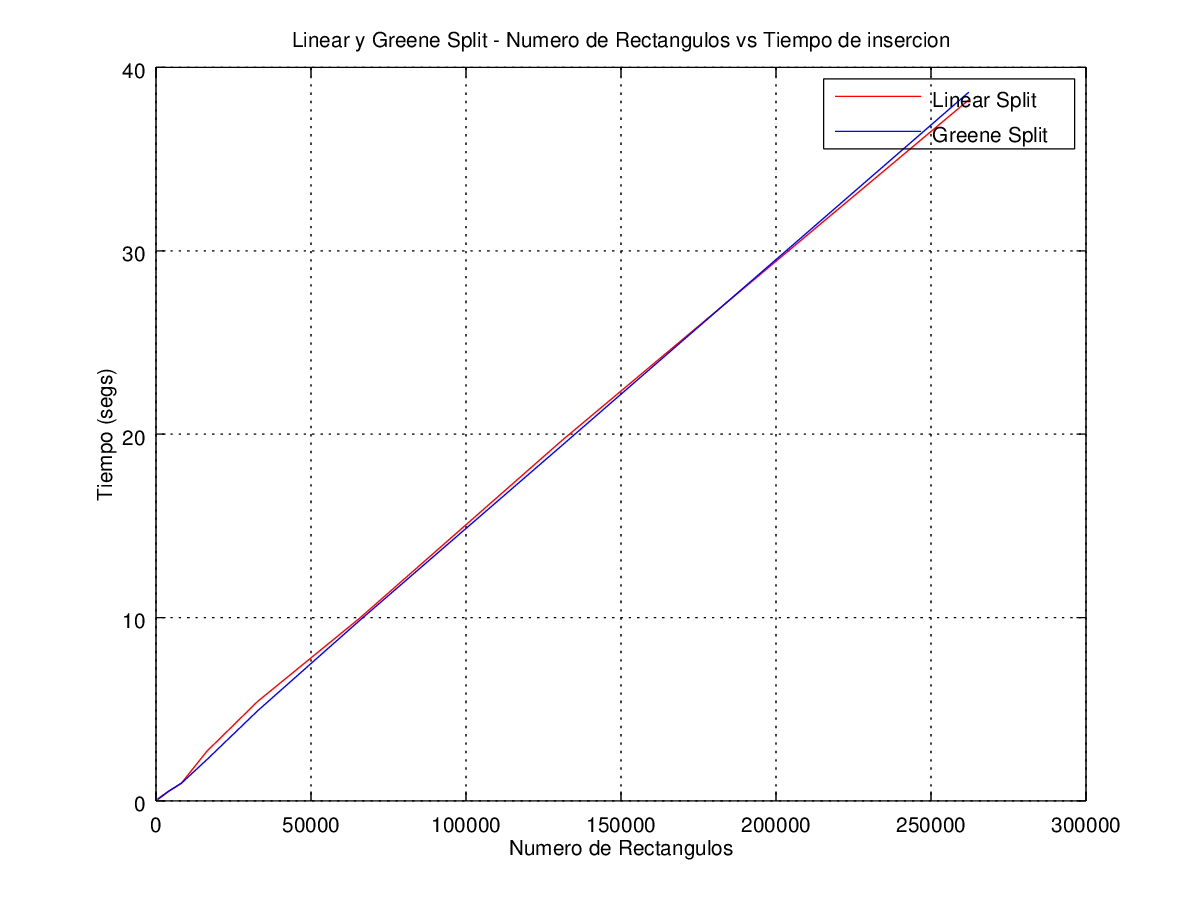
\includegraphics[width=0.75\textheight]{fig1.png}
	\end{center}

	% % % % % % % % % % % % % % % % % % % % % % % % % % % % % % % % % % % % % % % % % % % % % % % % % % % % % % % % % % % % % % % % % % % % % % % % % % % % % % % % % % % % % % % % % %
	\newpage
	% % % % % % % % % % % % % % % % % % % % % % % % % % % % % % % % % % % % % % % % % % % % % % % % % % % % % % % % % % % % % % % % % % % % % % % % % % % % % % % % % % % % % % % % % %

	\subsection{Espacio ocupado y porcentaje de llenado de páginas de disco}

	\begin{center}

		\begin{tabular}{|c|c|c|c|c|c|}
			\hline
			Rectángulos	& Nodos & Tamaño Total & Tamaño Promedio Nodo & \% llenado & Accesos a disco\\
			\hline
			$2^{9}$ 	& 18 & 16.5 KB & 956 bytes & 46,1\% & 102 \\
			\hline
			$2^{10}$ 	& 34 & 136 KB & 972 bytes & 47,6\% & 204 \\
			\hline
			$2^{11}$ 	& 68 & 272 KB & 982 bytes & 48,8\% & 408 \\
			\hline
			$2^{12}$ 	& 134 & 536 KB & 987 bytes & 49,5\% & 818 \\
			\hline
			$2^{13}$ 	& 266 & 1.1 MB & 990 bytes & 49,7\% & 1638 \\
			\hline
			$2^{14}$ 	& 530 & 2.1 MB & 992 bytes & 49,8\% & 3276 \\
			\hline
			$2^{15}$ 	& 1058 & 4.2 MB & 994 bytes & 50,0\% & 6552 \\
			\hline
			$2^{16}$ 	& 2116 & 8.4 MB & 995 bytes & 50,1\% & 13106 \\
			\hline
			$2^{17}$ 	& 4240 & 17 MB & 996 bytes & 50,1\% & 26214 \\
			\hline
			$2^{18}$ 	& 8458 & 34 MB & 996 bytes & 50,2\% & 52428 \\
			\hline
		\end{tabular}

		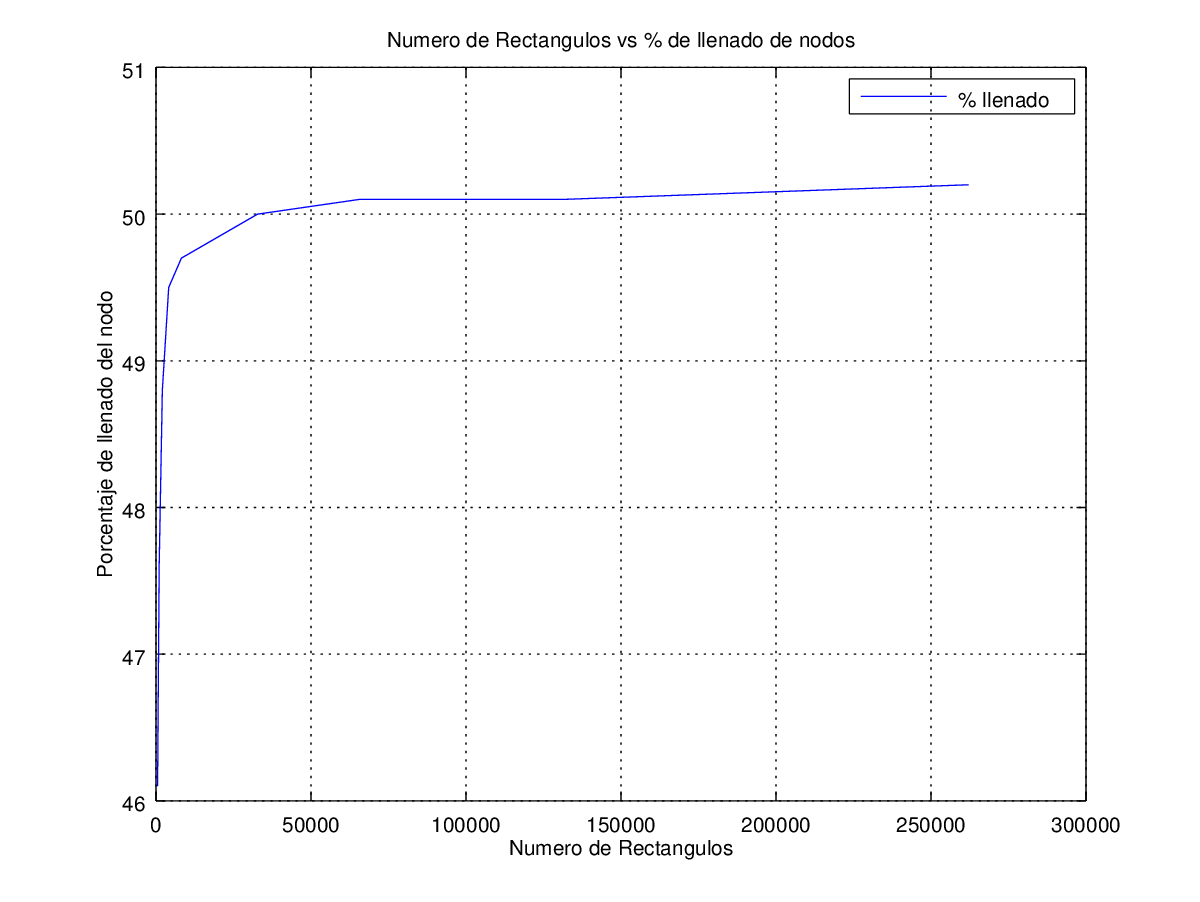
\includegraphics[width=0.55\textwidth]{fig2.png}

		(a) \% de llenado

		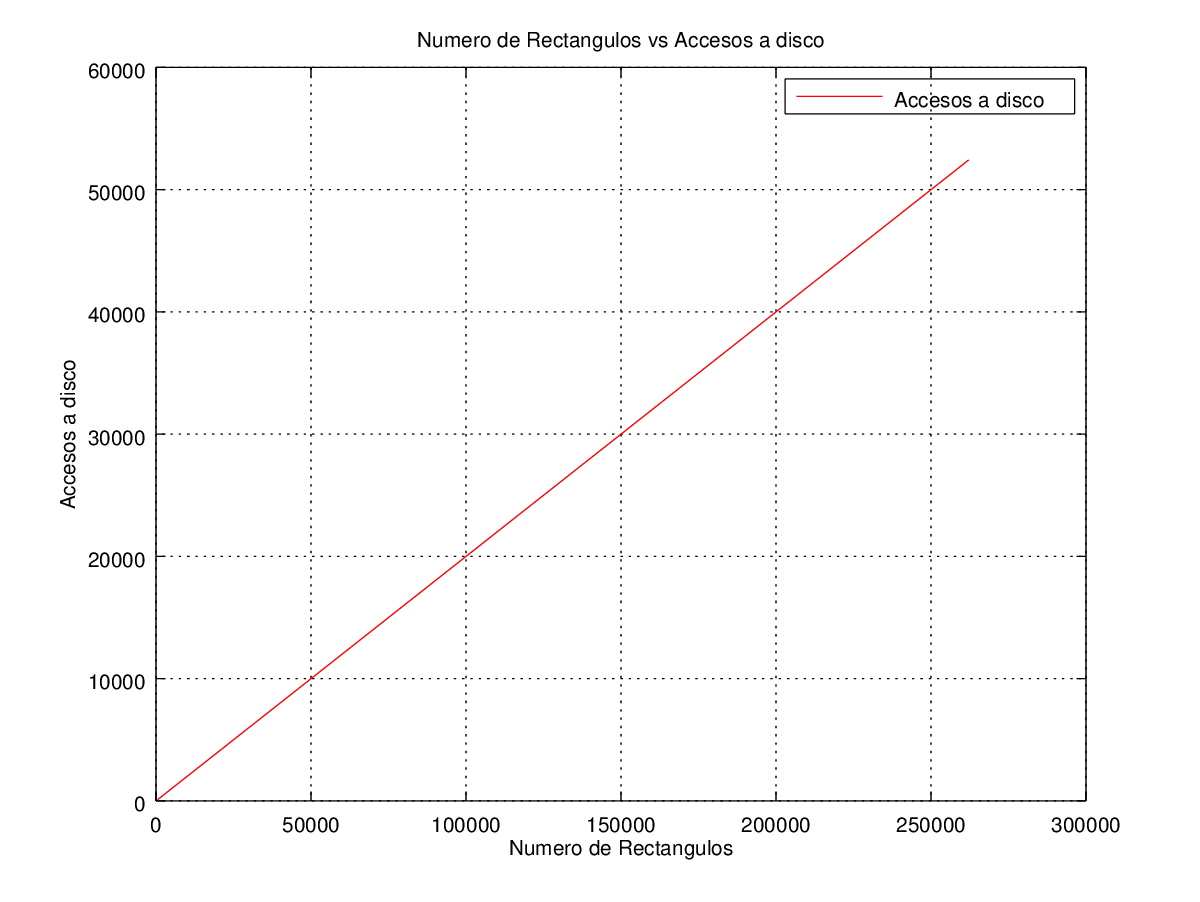
\includegraphics[width=0.55\textwidth]{fig4.png}

		(b) Accesos a disco


	\end{center}

	% % % % % % % % % % % % % % % % % % % % % % % % % % % % % % % % % % % % % % % % % % % % % % % % % % % % % % % % % % % % % % % % % % % % % % % % % % % % % % % % % % % % % % % % % %
	\newpage
	% % % % % % % % % % % % % % % % % % % % % % % % % % % % % % % % % % % % % % % % % % % % % % % % % % % % % % % % % % % % % % % % % % % % % % % % % % % % % % % % % % % % % % % % % %

	\subsection{Desempeño de operación \textit{Buscar}}

	\begin{center}

		\begin{tabular}{|c|c||c|}
			\hline
			Rectángulos	& Tiempo (seg) (Linear) & Tiempo (seg) (Greene) \\
			\hline
			$2^{9}/10$ 	& 0.002877	& 0.002891\\
			\hline
			$2^{10}/10$ 	& 0.005631	& 0.005252\\
			\hline
			$2^{11}/10$ 	& 0.011399	& 0.010876\\
			\hline
			$2^{12}/10$ 	& 0.022630	& 0.028296\\
			\hline
			$2^{13}/10$ 	& 0.045871	& 0.058527\\
			\hline
			$2^{14}/10$ 	& 0.116145	& 0.093235\\
			\hline
			$2^{15}/10$ 	& 0.717755	& 0.223559\\
			\hline
			$2^{16}/10$ 	& 0.495848	& 0.465250\\
			\hline
			$2^{17}/10$ 	& 0.832019	& 1.389346\\
			\hline
			$2^{18}/10$ 	& 2.194899	& 2.282709\\
			\hline
		\end{tabular}

		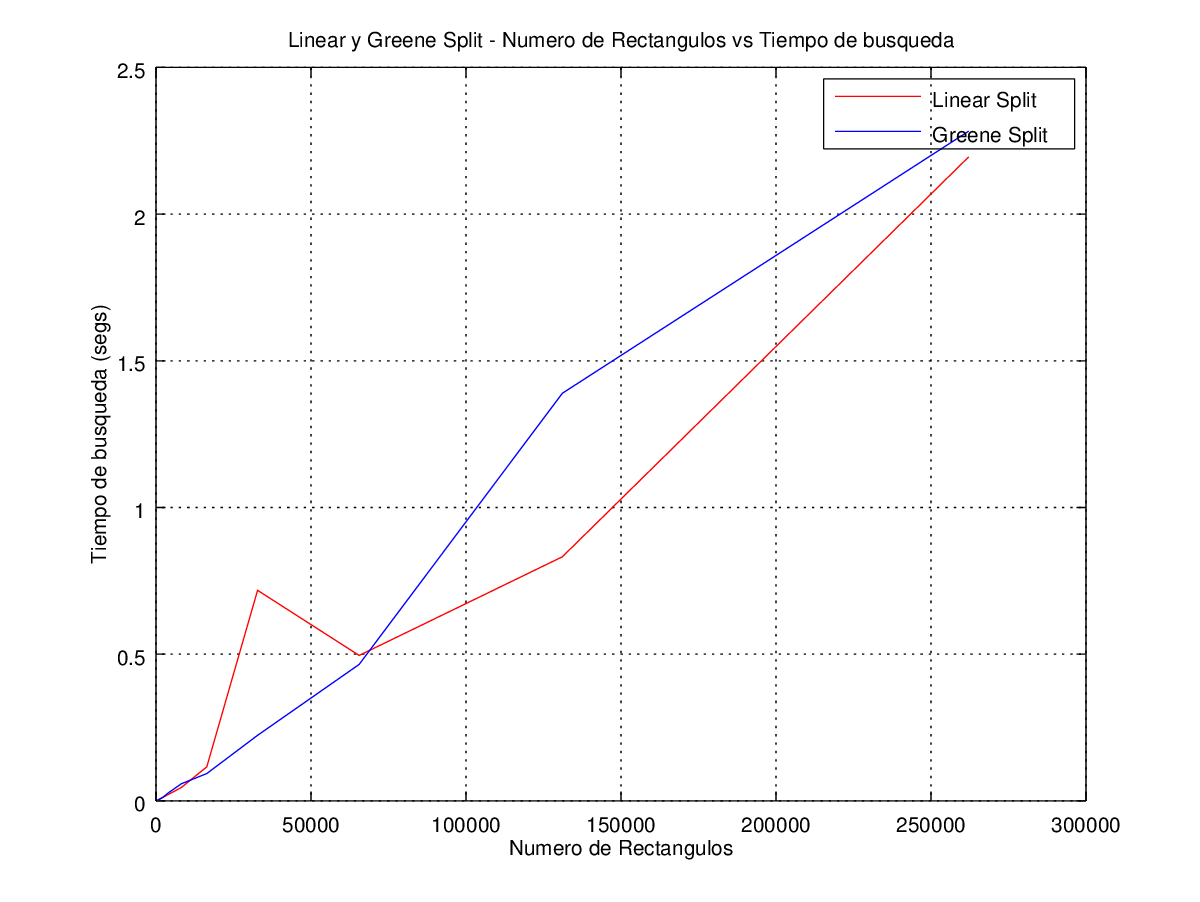
\includegraphics[width=0.75\textheight]{fig3.png}
	\end{center}

	% % % % % % % % % % % % % % % % % % % % % % % % % % % % % % % % % % % % % % % % % % % % % % % % % % % % % % % % % % % % % % % % % % % % % % % % % % % % % % % % % % % % % % % % % %
	\newpage
	% % % % % % % % % % % % % % % % % % % % % % % % % % % % % % % % % % % % % % % % % % % % % % % % % % % % % % % % % % % % % % % % % % % % % % % % % % % % % % % % % % % % % % % % % %

	\section{Análisis y Conclusiones}
% 	FIXME Análisis e Interpretación

	\subsection{Control de Overflow}

	En nuestra implementación, tanto Linear Split como Greene Split toman tiempos muy parecidos, lineal con respecto al número de rectángulos.

	Esto es, para al duplicar el número de rectángulos, se duplica también el tiempo, con una ventaja despreciable de Linear Split al inicio y de Greene Split al final.

	\subsection{Buscar}

	Un arreglo con control de Overflow Linear Split permite buscar ligeramente más rápido que uno con control de Overflow Greene Split, dado que comienzan a diverger en
	$n = 2^{16} = 65536$ rectángulos.

	\subsection{Conclusiones}

	El trabajo de un algoritmo en memoria secundaria es considerablemente más lento que uno en memoria principal. Sin embargo, a menudo se requiere trabajar con una cantidad de datos
	muy alta, lo que hace que cargarlos todos en memoria principal sea inviable.

	Para este caso, los experimentos realizados hacen que los rectángulos insertados y buscados ocupen tanta memoria que se requiere leer y escribir de disco.

	\begin{itemize}
		\item Según el análisis, tanto Linear Split como Greene Split muestran resultados parecidos, con una muy ligera ventaja de Linear Split.
		\item La búsqueda produce resultados un poco más apreciables, donde se muestra la ventaja que consiguió Linear Split.
		\item El uso de C facilitó el manejo preciso de memoria, pero aumentó considerablemente la complejidad para el algoritmo de uso correcto de la memoria, tanto
		principal como secundaria.
		\item Las inserciones, búsquedas y accesos a disco son $O(N)$
	\end{itemize}

\end{document}
